% =====================================================================
% Rozdział 6 – Testy i wyniki (WZÓR, ok. 6,5 strony)
% Styl bezosobowy. Liczby: wyniki potoku z 28.10.2026 (n = 92), badanie E4 (porownanie_rejestracji.csv),
% ocena U-Netu (n = 94), testy projekt/testy/test_systemu.py. Zestawienie: Claude outputs/dane_rozdz6/.
% Wymaga pakietów: booktabs, tabularx, makecell.
% Rysunki: rysunki/wyk_e4_tre.pdf, wyk_segmentacja.pdf, wyk_e2_tre.pdf, wyniki_para14.pdf, piksele_para14.png
% (wykresy: rysunki/wykresy_wyniki.py). Plan i zwroty: materialy/06_plan_zwroty_rozdzialy_4_7.md.
% TODO przed oddaniem: uruchom projekt/testy/uruchom_testy.bat (tab. tab:testy), wykonaj testy TG1–TG6,
% wpisz parametry komputera, na którym mierzono czasy (podrozdział sec:wyniki-rejestracja).
% =====================================================================

\chapter{Testy i wyniki}
\label{chap:testy}

W rozdziale przedstawiono protokół oceny, wyniki badania dokładności rejestracji (E1) i porównania metod rejestracji (E4), ocenę jakości segmentacji w obu modalnościach, zgodność obszarów między modalnościami bez adnotacji (badanie E2), parametry znamion i pikseli na obrazie termowizyjnym oraz wyniki testów funkcjonalnych. Rozdział zamyka dyskusja ograniczeń.

\section{Zbiór danych i protokół oceny}
\label{sec:protokol}

Badania przeprowadzono na zbiorze 94 par obrazów 34 znamion (podrozdział~\ref{sec:dane}). System przeanalizował 92 pary. W parach 75 i 76 maska znacznika wykryta na zdjęciu nie miała poprawnego otworu (otwór stanowił 2\% i 8\% otoczki wypukłej wobec oczekiwanych 15--60\%), a ponowna detekcja dała obiekt niezgodny z wzorcem $\Pi$ (zgodność 0,54 i 0,58 przy progu 0,65). Nie można było więc wyznaczyć obszaru segmentacji znamienia i zgodnie z wymaganiem WN6 analiza zakończyła się komunikatem, a nie błędnym wynikiem. Wzorcem do oceny były adnotacje z programu CVAT, których system nie wykorzystuje w trakcie analizy. Przed wykonaniem badań przyjęto kryteria akceptacji z rozdziału~\ref{chap:analiza}: czas rejestracji krótszy niż 15~s (WN1), mediana błędu TRE nie większa niż 1~mm (WN4) i współczynnik Dice'a segmentacji znacznika na obrazie termowizyjnym co najmniej 0,9 (WN5).

Ze względu na skośne rozkłady błędów podano medianę i zakres wartości, a obok nich średnią i odchylenie standardowe. Wyniki dwóch metod uzyskane na tych samych parach porównywano testem Wilcoxona dla par wiązanych, a zależność dwóch miar oceniano współczynnikiem korelacji rang Spearmana~$\rho$.

\section{Dokładność rejestracji}
\label{sec:wyniki-rejestracja}

W badaniu E1 narożniki i obrys znacznika oznaczone na zdjęciu przeniesiono macierzą $T$ wyznaczoną przez system i porównano z oznaczonymi na obrazie termowizyjnym (tab.~\ref{tab:e1-e2}, kolumna E1). Mediana błędu TRE wyniosła 0,61~mm, a w 78 z 92 par (85\%) średni błąd narożników nie przekroczył 1~mm -- wymaganie WN4 zostało spełnione. Średnia (0,96 $\pm$ 2,52~mm) jest zawyżona przez jedną parę: w parze 78 rejestracja nie powiodła się (TRE 24,7~mm). Kolejne największe błędy wystąpiły w parach 8 (2,3~mm), 79 (1,9~mm) i 72 (1,7~mm). Rozmiar piksela obrazu termowizyjnego na skórze wynosił 0,21--0,44~mm (mediana 0,28~mm), typowy błąd rejestracji odpowiada więc około dwóm pikselom kamery termowizyjnej.

\begin{table}[htbp]
  \centering
  \caption{Zgodność znacznika po rejestracji: E1 -- obrys i narożniki z CVAT na zdjęciu przeniesione macierzą $T$ względem oznaczonych na obrazie termowizyjnym; E2 -- maska folii ze zdjęcia przeniesiona macierzą $T$ względem maski z modelu M3, bez adnotacji; mediana (min.--maks.), $n = 92$}
  \label{tab:e1-e2}
  \small
  \begin{tabular}{lcc}
    \toprule
    Miara & E1 (wzorzec CVAT) & E2 (model M3) \\
    \midrule
    TRE -- średni błąd narożników [mm] & 0,61 (0,29--24,69) & -- \\
    TRE -- największy błąd narożnika [mm] & 1,13 (0,44--43,85) & -- \\
    Dice znacznika & 0,960 (0,548--0,979) & 0,966 (0,719--0,980) \\
    IoU znacznika & 0,923 (0,377--0,959) & 0,934 (0,562--0,960) \\
    HD95 znacznika [mm] & 0,81 (0,28--19,57) & 0,75 (0,42--8,97) \\
    ASSD znacznika [mm] & 0,32 (0,16--5,63) & 0,25 (0,14--2,17) \\
    Dice otworu (ROI) & 0,960 (0,545--0,983) & 0,960 (0,597--0,980) \\
    HD95 otworu [mm] & 0,75 (0,30--11,55) & 0,88 (0,44--6,59) \\
    \bottomrule
  \end{tabular}
\end{table}

W badaniu E4 porównano metodę zastosowaną w systemie z rejestracją opartą na informacji wzajemnej~\cite{zitova2003} (metryka \texttt{MattesMutualInformation} biblioteki SimpleITK, stosowana we wcześniejszej wersji systemu) w dwóch wariantach: na całym obrazie i w otoczeniu znacznika. Wszystkie metody startowały z tego samego dopasowania wstępnego, a ich dokładność oceniano błędem TRE (rys.~\ref{fig:e4}). Rejestracja na maskach znacznika osiągnęła medianę TRE 0,61~mm (rozstęp międzykwartylowy 0,52--0,78~mm) i błąd nie większy niż 1~mm w 79 z 92 par. Informacja wzajemna w otoczeniu znacznika dała medianę 3,36~mm (13 par z błędem do 1~mm), a na całym obrazie -- 4,51~mm (5 par). Metoda zastosowana w systemie dała mniejszy błąd niż lepszy z wariantów informacji wzajemnej w 87 z 92 par (test Wilcoxona, $p < 0{,}001$). Informacja wzajemna nie poprawiła nawet dopasowania wstępnego (mediana 3,13~mm), co jest zgodne z obserwacją, że intensywności obrazu widzialnego i termowizyjnego nie są ze sobą bezpośrednio powiązane~\cite{visible-and-infared}, a funkcja informacji wzajemnej może mieć wiele maksimów~\cite{correlation-ratio}.

\begin{figure}[htbp]
  \centering
  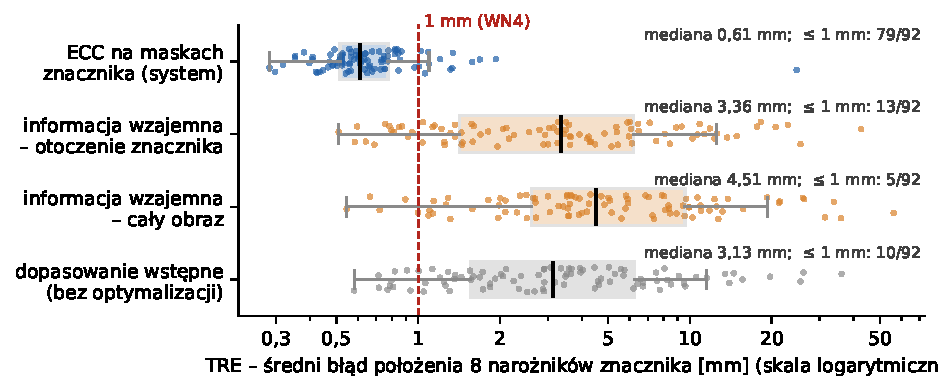
\includegraphics[width=0.92\textwidth]{rysunki/wyk_e4_tre.pdf}
  \caption{Błąd TRE czterech metod rejestracji w badaniu E4 ($n = 92$ pary); punkty -- pary, prostokąt -- kwartyle, czarna linia -- mediana. Źródło: opracowanie własne}
  \label{fig:e4}
\end{figure}

Mediana czasu rejestracji metodą zastosowaną w systemie wyniosła 8,4~s (maksymalnie 13,2~s), wobec 10,5~s i 16,0~s dla wariantów informacji wzajemnej; wymaganie WN1 zostało spełnione. % TODO: dopisać procesor i pamięć komputera, na którym mierzono czasy.

\section{Jakość segmentacji w obu modalnościach}
\label{sec:wyniki-segmentacja}

Jakość segmentacji oceniono względem masek z programu CVAT (tab.~\ref{tab:segmentacja}, rys.~\ref{fig:segmentacja}). Model M3 w 5-krotnej walidacji krzyżowej według znamion uzyskał współczynnik Dice'a 0,969 $\pm$ 0,008 (minimum 0,937), a wartości w poszczególnych foldach mieściły się w zakresie 0,968--0,970. Współczynnik Dice'a był nie mniejszy niż 0,9 dla wszystkich 94 obrazów, więc wymaganie WN5 zostało spełnione. Model zachowuje pole znacznika (stosunek pól 1,004), a mediana HD95 wynosi 0,62~mm, czyli około dwa piksele obrazu termowizyjnego. Detektor klasyczny z modułu rejestracji uzyskał mniejszy współczynnik Dice'a (0,954 $\pm$ 0,017; test Wilcoxona, $p < 0{,}001$) i zaniżał pole folii (stosunek pól 0,950), co uzasadnia zastosowanie modelu uczonego jako niezależnego punktu odniesienia w badaniu E2.

\begin{table}[htbp]
  \centering
  \caption{Segmentacja względem adnotacji z CVAT: średnia $\pm$ odchylenie standardowe (mediana)}
  \label{tab:segmentacja}
  \small
  \begin{tabular}{lccc}
    \toprule
    Miara & \makecell{M1 -- znamię,\\ zdjęcie ($n = 92$)} & \makecell{M3 -- znacznik,\\ termowizja ($n = 94$)} & \makecell{detektor klasyczny,\\ termowizja ($n = 94$)} \\
    \midrule
    Dice & 0,870 $\pm$ 0,103 (0,896) & 0,969 $\pm$ 0,008 (0,970) & 0,954 $\pm$ 0,017 (0,959) \\
    IoU & 0,782 $\pm$ 0,129 (0,812) & 0,939 $\pm$ 0,015 (0,941) & 0,913 $\pm$ 0,031 (0,921) \\
    HD95 [mm] & 0,38 $\pm$ 0,53 (0,24) & 0,68 $\pm$ 0,27 (0,62) & 1,06 $\pm$ 0,59 (0,83) \\
    ASSD [mm] & 0,15 $\pm$ 0,22 (0,10) & 0,23 $\pm$ 0,06 (0,22) & 0,32 $\pm$ 0,12 (0,31) \\
    stosunek pól & 1,22 $\pm$ 0,59 (1,10) & 1,004 $\pm$ 0,030 (1,006) & 0,950 $\pm$ 0,044 (0,951) \\
    \bottomrule
  \end{tabular}
\end{table}

% OPCJA (ok. 0,4 s.): wykres powtarza dane z tab. tab:segmentacja w postaci rozkładów -- przy braku miejsca usuń.
\begin{figure}[htbp]
  \centering
  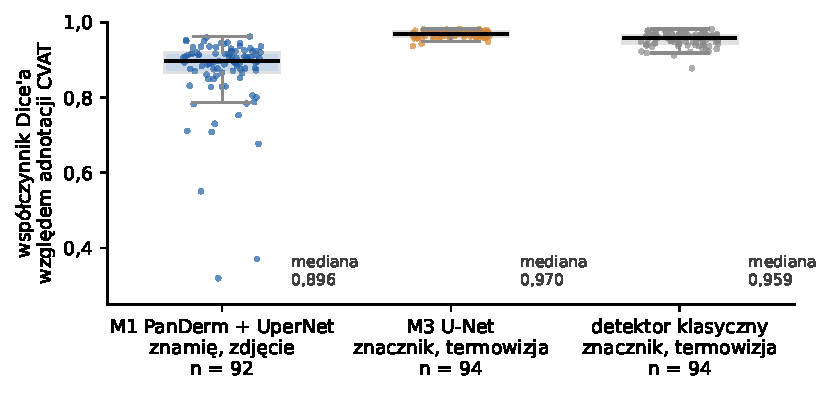
\includegraphics[width=0.85\textwidth]{rysunki/wyk_segmentacja.pdf}
  \caption{Współczynnik Dice'a segmentacji względem adnotacji z CVAT; punkty -- pary obrazów. Źródło: opracowanie własne}
  \label{fig:segmentacja}
\end{figure}

Model M1 na zdjęciach z telefonu uzyskał współczynnik Dice'a 0,870 $\pm$ 0,103 (mediana 0,896), a więc niewiele mniejszy niż na zbiorze testowym ISIC (0,899), mimo przesunięcia dziedziny. W 81 z 92 par współczynnik był nie mniejszy niż 0,8. Najsłabsze wyniki dotyczyły znamion położonych przy krawędzi folii lub w jej cieniu (pary 57 i 81: 0,32 i 0,37) oraz bardzo bladego znamienia (para 59: 0,55). Mediana stosunku pól równa 1,10 oznacza, że model systematycznie zawyża obszar znamienia, głównie przez szerszy niż w adnotacji brzeg. Znamiona są małe (mediana średnicy 2,1~mm), a dla małych struktur miary pokrycia są bardzo wrażliwe na błąd pojedynczych pikseli~\cite{maierhein2024}; dlatego obok współczynnika Dice'a podano miary odległościowe, z których wynika, że typowe przesunięcie brzegu maski (mediana ASSD) wynosi 0,10~mm.

\section{Zgodność obszaru zainteresowania między modalnościami}
\label{sec:wyniki-e2}

Badanie E2 nie wymaga adnotacji, dlatego system wykonuje je dla każdej analizowanej pary. Maska folii ze zdjęcia, przeniesiona macierzą $T$, pokrywała się z maską z modelu M3 ze współczynnikiem Dice'a 0,957 $\pm$ 0,032 (mediana 0,966), a w 89 z 92 par współczynnik był nie mniejszy niż 0,9 (tab.~\ref{tab:e1-e2}, kolumna E2). Dla otworu znacznika, czyli obszaru zainteresowania, mediana współczynnika Dice'a wyniosła 0,960, mediana HD95 -- 0,88~mm, a mediana przesunięcia środków -- 0,23~mm. Przykład dla pary 14 przedstawiono na rysunku~\ref{fig:wyniki-para}.

\begin{figure}[htbp]
  \centering
  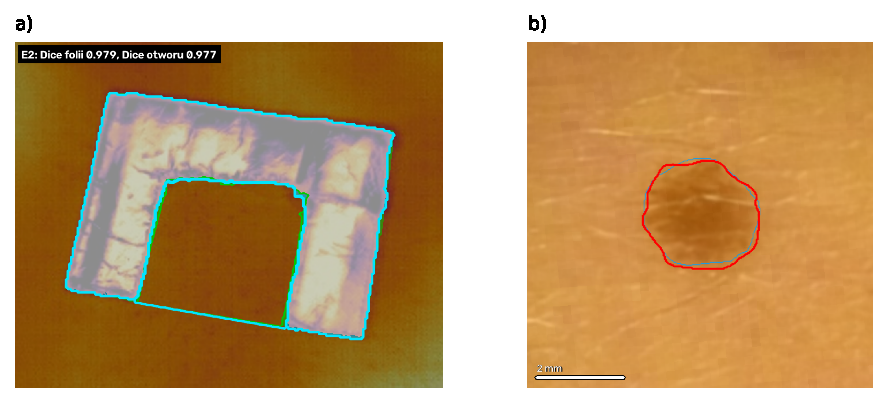
\includegraphics[width=0.9\textwidth]{rysunki/wyniki_para14.pdf}
  \caption{Para 14: a)~maska folii ze zdjęcia przeniesiona macierzą $T$ i maska z modelu M3 (biały -- obie maski, zielony -- tylko ze zdjęcia, turkusowy -- tylko M3), b)~nałożenie obrazu termowizyjnego na zdjęcie w otoczeniu znamienia: maska M1 (czerwona) i adnotacja z CVAT (niebieska); widoczne kwadraty to piksele kamery termowizyjnej. Źródło: opracowanie własne}
  \label{fig:wyniki-para}
\end{figure}

Najważniejszą właściwością badania E2 jest to, że wykrywa ono nieudaną rejestrację bez wzorca. Współczynnik Dice'a folii w badaniu E2 jest silnie skorelowany z błędem TRE wyznaczonym względem adnotacji ($\rho = -0{,}72$; rys.~\ref{fig:e2-tre}). Najmniejsze wartości wystąpiły w parach o największym błędzie rejestracji: 78 (Dice 0,72, TRE 24,7~mm), 8 (0,86; 2,3~mm) i 79 (0,89; 1,9~mm). Współczynnik Dice'a otworu mniejszy niż 0,93 wystąpił w 10 parach, z których 9 miało TRE większe niż 1~mm. Trafne okazało się też ostrzeżenie o niepewnej detekcji znacznika: wszystkie cztery pary, w których zgodność kształtu znacznika na zdjęciu z wzorcem była mniejsza niż 0,65 (pary 8, 59, 78 i 79), miały TRE większe niż 1,3~mm. Badanie E2 ujawnia również błędy segmentacji w jednej z modalności: w parze 1 maska folii ze zdjęcia wchodziła w otwór znacznika, co obniżyło współczynnik Dice'a otworu do 0,81 przy poprawnej rejestracji.

\begin{figure}[htbp]
  \centering
  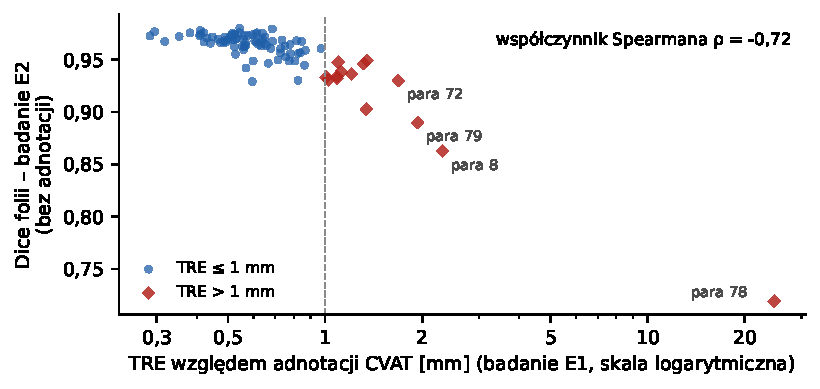
\includegraphics[width=0.9\textwidth]{rysunki/wyk_e2_tre.pdf}
  \caption{Współczynnik Dice'a folii w badaniu E2 (bez adnotacji) a błąd TRE względem adnotacji (badanie E1), $n = 92$ pary. Źródło: opracowanie własne}
  \label{fig:e2-tre}
\end{figure}

\section{Parametry znamion i piksele na obrazie termowizyjnym}
\label{sec:wyniki-piksele}

Parametry znamion zmierzone przez system oraz charakterystykę pikseli znamion na obrazie termowizyjnym zestawiono w tabeli~\ref{tab:znamiona}. Znamiona w zbiorze były małe: mediana pola wyniosła 3,4~mm$^2$, a średnicy równoważnej -- 2,1~mm. Stosunek pola znamienia przeniesionego na obraz termowizyjny do pola zmierzonego na zdjęciu wyniósł 1,015 $\pm$ 0,034. Oba pola obliczono niezależnymi homografiami, więc wynik bliski jedności potwierdza spójność skali i rejestracji.

\begin{table}[htbp]
  \centering
  \caption{Parametry znamion i piksele znamion na obrazie termowizyjnym ($n = 92$)}
  \label{tab:znamiona}
  \small
  \begin{tabular}{lcc}
    \toprule
    Wielkość & Mediana & Min.--maks. \\
    \midrule
    pole znamienia, model M1 [mm$^2$] & 3,42 & 1,16--28,58 \\
    pole znamienia, adnotacja CVAT [mm$^2$] & 3,24 & 0,97--28,09 \\
    średnica równoważna [mm] & 2,09 & 1,22--6,03 \\
    maksymalna średnica Fereta [mm] & 2,65 & 1,40--8,48 \\
    kolistość & 0,819 & 0,237--0,867 \\
    pole na obrazie termowizyjnym / pole na zdjęciu & 1,020 & 0,767--1,069 \\
    piksele w masce znamienia & 44 & 10--290 \\
    piksele pokryte częściowo (ułamek $< 0{,}5$) & 12 & 3--38 \\
    odchylenie standardowe intensywności w znamieniu [j.s.] & 14,1 & 6,0--68,4 \\
    rozstęp intensywności w znamieniu [j.s.] & 65 & 27--333 \\
    \bottomrule
  \end{tabular}
  \\[2pt]{\footnotesize j.s. -- jednostki surowe detektora (wartości z nagrania .SEQ)}
\end{table}

Dla 92 znamion zapisano łącznie 7337 pikseli należących do masek oraz piksele pokryte częściowo, wraz ze współrzędnymi i surową intensywnością (WF15). Przykład przedstawiono na rysunku~\ref{fig:piksele}. Zmienność intensywności w obrębie znamienia była niewielka: mediana odchylenia standardowego wyniosła 14,1 jednostek surowych. Na podstawie map temperatur wyznaczonych z parametrów kamery jednej jednostce stopnia Celsjusza odpowiada w zakresie temperatur skóry (30--37~°C) około 213 jednostek surowych, więc odchylenie to odpowiada około 0,07~°C. Wynik ten jest zgodny z obserwacją, że bez schłodzenia skóry znamię nie wyróżnia się na obrazie termowizyjnym~\cite{visualization-detection-cancer}. Należy też pamiętać, że przy medianie błędu rejestracji około dwóch pikseli kamery piksele brzegowe mogą obejmować skórę wokół znamienia; dlatego dla każdego piksela zapisywany jest ułamek pokrycia.

\begin{figure}[htbp]
  \centering
  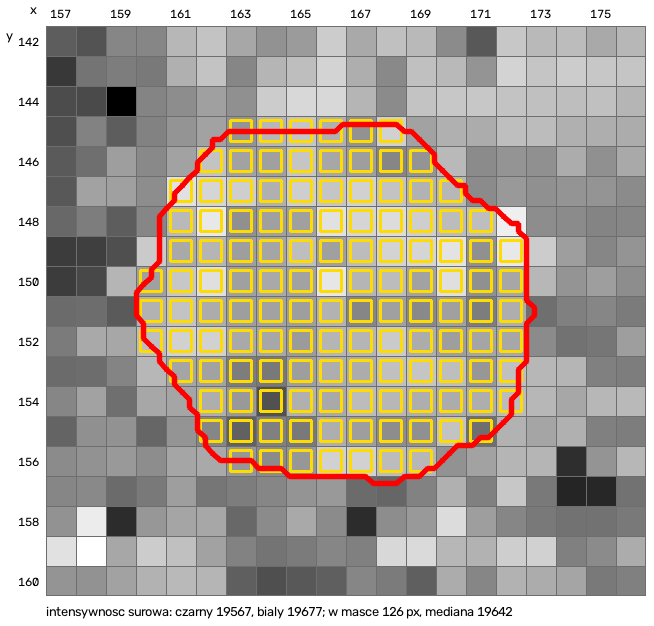
\includegraphics[width=0.5\textwidth]{rysunki/piksele_para14.png}
  \caption{Piksele obrazu termowizyjnego objęte znamieniem w parze 14: surowa intensywność z nagrania (skala szarości rozciągnięta w kadrze), znamię przeniesione ze zdjęcia (czerwona linia) i piksele w masce (żółte ramki); na brzegach współrzędne $x$ i $y$ pikseli. Źródło: opracowanie własne}
  \label{fig:piksele}
\end{figure}

\section{Testy funkcjonalne}
\label{sec:testy-funkcjonalne}

Spełnienie wymagań funkcjonalnych i części wymagań pozafunkcjonalnych sprawdzono 18 testami automatycznymi napisanymi z użyciem modułu \texttt{unittest} (tab.~\ref{tab:testy}). Testy wykonują etapy systemu bez interfejsu graficznego na danych ze zbioru (para 14 z adnotacjami i para 75 z niewykrywalnym znacznikiem) oraz na danych przygotowanych w teście, a wyniki zapisują w folderach tymczasowych i osobnej bazie danych. Zaliczono 17 testów; test T09 pominięto, ponieważ w środowisku testowym nie było wag modelu M3. Czas wykonania całego zestawu wyniósł około 20~s. % TODO: uruchom projekt/testy/uruchom_testy.bat i wpisz wynik (w maszynie bez wag U-Net: 17 zaliczonych, T09 pominięty).

\begin{table}[htbp]
  \centering
  \caption{Testy funkcjonalne systemu}
  \label{tab:testy}
  \footnotesize
  \begin{tabularx}{\textwidth}{l l X l}
    \toprule
    ID & Wymaganie & Sprawdzane zachowanie & Wynik \\
    \midrule
    T01 & WF1 & wczytanie pary ze zbioru: obrazy, numer znamienia, adnotacje & zaliczony \\
    T02 & WF1, WN6 & nieistniejący plik -- komunikat zamiast awarii & zaliczony \\
    T03 & WN6 & etap wywołany przed poprzednim -- komunikat & zaliczony \\
    T04 & WF2, WN1, WN4 & pełna rejestracja pary 14: czas 6,4~s, TRE 0,69~mm & zaliczony \\
    T05 & WN6 & obraz termowizyjny bez znacznika -- ostrzeżenie (zgodność z $\Pi$ 0,54) & zaliczony \\
    T06 & WN6 & para 75 -- znacznik niezgodny z wzorcem odrzucony z komunikatem & zaliczony \\
    T07 & WF4 & 8 narożników w obu modalnościach, IoU wzorca $\geq 0{,}8$ & zaliczony \\
    T08 & WF7, WF8 & pole znamienia na obu obrazach zgodne ($\pm$15\%), komplet parametrów & zaliczony \\
    T09 & WF6, WF9 & maska M3 i miary E2 (Dice folii $\geq 0{,}9$) & pominięty$^{*}$ \\
    T10 & WF15 & współrzędne i surowa intensywność pikseli zgodne z nagraniem & zaliczony \\
    T11 & WF15 & zapis pikseli do CSV i odczyt bez utraty danych & zaliczony \\
    T12 & WF15, WN6 & brak nagrania .SEQ -- analiza bez pikseli, uwaga w raporcie & zaliczony \\
    T13 & WF15 & własne pliki z nagraniem .SEQ -- odczyt intensywności & zaliczony \\
    T14 & WF11 & raport HTML, \texttt{metryki.json}, obrazy PNG i CSV pikseli & zaliczony \\
    T15 & WF12, WN9 & zapis analizy, miar i pikseli w bazie & zaliczony \\
    T16 & WF12 & migracja bazy ze starszej wersji schematu & zaliczony \\
    T17 & WF9 & miary zgodności na maskach o znanym wyniku & zaliczony \\
    T18 & WF7 & przeniesienie punktów i ułamek pokrycia pikseli & zaliczony \\
    \bottomrule
  \end{tabularx}
  \\[2pt]{\footnotesize $^{*}$ wymaga wag modelu M3, niedostępnych w środowisku testowym; % TODO: po uruchomieniu uruchom_testy.bat na komputerze autora wpisać wynik
}
\end{table}

Działanie interfejsu graficznego sprawdzono ręcznie według scenariuszy: wczytanie pary ze zbioru i własnych plików (TG1), wykonanie wszystkich etapów jednym poleceniem (TG2), praca krok po kroku z kontrolą aktywności przycisków (TG3), regulacja przezroczystości i zapis nałożenia (TG4), wyświetlanie objaśnień wielkości (TG5) oraz zapis i otwarcie raportu wraz z podglądem obrazów (TG6). % TODO: wykonać TG1–TG6 i wpisać wynik (np. „Wszystkie scenariusze zakończyły się zgodnie z oczekiwaniami.”).

\section{Dyskusja i ograniczenia}
\label{sec:dyskusja}

Zastosowanie znacznika widocznego w obu modalnościach i maksymalizacja kryterium ECC na maskach zamiast na intensywnościach zmniejszyły medianę błędu rejestracji około pięciokrotnie względem informacji wzajemnej. Bezpośrednie porównanie z wynikami innych prac jest ograniczone, ponieważ stosowano w nich inne dane i miary: błąd w pikselach przy rejestracji z szablonem kalibracyjnym~\cite{non-contact-breathing-monitoring}, zgodność masek dużych obiektów (stóp)~\cite{gonzalezperez2021} albo miary podobieństwa obrazów bez błędu położenia punktów w milimetrach~\cite{oniga2026}. W niniejszej pracy błąd rejestracji wyrażono w milimetrach na płaszczyźnie znacznika, a dodatkowo zastosowano niezależną kontrolę bez adnotacji (E2), która pozwala wskazać pary wymagające sprawdzenia.

Ograniczenia przeprowadzonych badań są następujące:
\begin{itemize}
  \item dane pochodzą z jednej serii pomiarowej, jednego zestawu urządzeń i jednej osoby wykonującej zdjęcia, a adnotacje wykonał jeden oznaczający -- zgodność ekspertów przy oznaczaniu znamion jest ograniczona~\cite{codella2019};
  \item model przekształcenia zakłada, że skóra w obrębie znacznika jest płaska; znacznik musi w całości znajdować się w kadrze obu urządzeń;
  \item obraz termowizyjny bez znacznika powoduje ostrzeżenie, ale nie przerywa rejestracji (test T05) -- decyzję podejmuje użytkownik na podstawie uwag w raporcie;
  \item model M1 zawyża pole znamienia (mediana stosunku pól 1,10), a jego jakość na zdjęciach z telefonu oceniono tylko na 92 parach;
  \item intensywność pikseli jest surową wartością detektora, bez kalibracji temperatury i bez schłodzenia skóry, więc nie pozwala ocenić termicznych właściwości znamienia.
\end{itemize}
